\documentclass[11pt]{article}
%\usepackage[14pt]{extsizes} % для того чтобы задать нестандартный 14-ый размер шрифта
%\usepackage[utf8]{inputenc}
\usepackage{mathtext}
\usepackage[english, russian]{babel}
\usepackage{amsmath}
\usepackage{amsfonts}
\usepackage{float}
\usepackage[margin=0.8in]{geometry}
\usepackage{multirow}
\usepackage{graphicx}
\usepackage[utf8x]{inputenc} % указать кодировку русского текста
\usepackage{fancyhdr}
\usepackage{indentfirst} % отступ в первой строке абзаца
\usepackage{wrapfig}
\usepackage{placeins}
\usepackage{wrapfig}
\usepackage{caption}
\usepackage{amssymb}
\usepackage{mathtools}
\usepackage[thinc]{esdiff}
\usepackage{cmap}
\usepackage[table,xcdraw]{xcolor}

\pagestyle{fancy}
\begin{document}

\begin{titlepage}
\begin{center}
%\vspace*{1cm}
\large{\small ФЕДЕРАЛЬНОЕ ГОСУДАРСТВЕННОЕ АВТОНОМНОЕ ОБРАЗОВАТЕЛЬНОЕ\\ УЧРЕЖДЕНИЕ ВЫСШЕГО ОБРАЗОВАНИЯ\\ МОСКОВСКИЙ ФИЗИКО-ТЕХНИЧЕСКИЙ ИНСТИТУТ\\ (НАЦИОНАЛЬНЫЙ ИССЛЕДОВАТЕЛЬСКИЙ УНИВЕРСИТЕТ)\\ ФИЗТЕХ-ШКОЛА РАДИОТЕХНИКИ И КОМПЬЮТЕРНЫХ ТЕХНОЛОГИЙ}
\vfill
\line(1,0){430}\\[1mm]
\huge{Лабораторная работа 3.2.4}\\
\huge\textbf{Свободные колебания в электрическом контуре}\\
\line(1,0){430}\\[1mm]
\vfill
\begin{flushright}
\normalsize{Устюжанина Мария}\\
\normalsize{\textbf{Группа Б01-107}}\\
\end{flushright}
\end{center}
\end{titlepage}
\fancyhead[L] {Работа 3.2.4}

\par \textbf{Цель работы:} Исследование свободных колебаний в электрическом колебательном контуре.

\par \textbf{В работе используются:} генератор импульсов, электронное реле, магазин сопротивлений, магазин емкостей, катушка индуктивности, электронный осциллограф, измеритель LRC. 


\section{Теоретическая часть:} 

\subsection*{Свободные колебания}
Рассмотрим электрический контур, состоящий из последовательно соединённых конденстора $C$, катушки индуктивности $L$ и резистора $R$. Обозначим разность потенциалов на конденсаторе $U_C$, а ток, текущий в контуре, через $I$. Второе првило Кирхгофа:
\begin{equation}
L \dfrac{d^2I}{dt^2}+R\dfrac{dI}{dt}+\dfrac{I}{C}=0.
\end{equation}
Вводя обозначения $\gamma = \dfrac{R}{2L}$, $\omega_0^2=\dfrac{1}{LC}$, получим уравнение
\begin{equation}
\ddot{I}+2\gamma\dot{I}+\omega_0^2I=0.
\end{equation}
Его решение в общем виде:
\begin{equation}
I = -\dfrac{U_0}{L\kappa}e^{-\gamma t}\text{sh}(\kappa t), 
\end{equation}
где $\kappa = \sqrt{\gamma^2 - \omega_0^2}$, $U_0 = U_C$ -- начальное напряжение на конденсаторе.

\subsection*{Затухающие колебания}
 В случае, когда $\gamma < \omega_0$, имеем $\kappa = i\omega$, где $\omega = \sqrt{\omega_0^2 - \gamma^2}$ -- \textit{частоты свободных (собственных) колебаний}. Тогда ток
 \begin{equation}
 I = -\dfrac{U_0}{L\omega}e^{-\gamma t}\sin(\omega t)
 \end{equation}
 затухает и имеет колебательный характер. Величина $\gamma$ определяет затухание колебаний: $\gamma = \dfrac{1}{\tau}$, где $\tau$ -- время затухание амплитуды в $e$ раз.
Формулы для наряжение на кондесаторе и тока в цепи можно переписать иначе:
\begin{equation}
\begin{array}{c}
U_C = U_0 \dfrac{\omega_0}{\omega}e^{-\gamma t} \cos(\omega t - \theta),\\
\\
I = -\dfrac{U_0}{L}e^{-\gamma t} \cos(\omega t - \theta).
\end{array}
\end{equation}

\subsection*{Апериодические колебания}
В случае $\gamma > \omega_0$, формулы для тока и напряжения на конденсаторе имеют следующий вид:
$$
\begin{array}{c}
I = -\dfrac{U_0}{L\kappa}e^{-\gamma t}\text{sh}(\kappa t),\\
\\
U_C = U_0 e^{-\gamma t}\left( \dfrac{\gamma}{\kappa}\text{sh}(\kappa t) + \text{ch}(\kappa t) \right).
\end{array}
$$
Процесс в этом случае не является колебательным, его называют апериодическим. Режим, соответствующий $\gamma = \omega_0$, называются \textit{критическим}. В этом случае предельный переход $\omega \rightarrow 0$ в $(5)$ даст 
$$
\begin{array}{c}
I = -\dfrac{U_0}{L}te^{-\gamma t},\\
\\
U_C=U_0 e^{-\gamma t}(1+\gamma t).
\end{array}
$$
Сопротивление в этом случае 
\begin{equation}
R_{\text{кр}}= 2 \sqrt{\dfrac{L}{C}}
\end{equation}
называется \textit{критическим сопротивлением} контура.\\
\textit{Добротность} контура по определению 
$$
Q = 2\pi \dfrac{W}{\Delta W},
$$ 
где $W$ -- запасённая энергия, $\Delta W$ -- потери за период. Тогда
$$
Q = 2\pi\dfrac{CU_0^2/2 \cdot e^{-2\gamma t}}{CU_0^2/2 \cdot (e^{-2\gamma t} - e^{-2\gamma (T+t)})}=\dfrac{\pi}{\gamma T}=\dfrac{1}{R}\sqrt{\dfrac{L}{C}}.
$$
\textit{Логарифмическим декрементом затухания} называются число
$$
\Theta = \text{ln}\dfrac{U_k}{U_{k+1}}=\text{ln} e^{\gamma T}=\gamma T
$$
или 
$$
\Theta = \dfrac{1}{n} \text{ln}\dfrac{U_k}{U_{k+n}}.
$$
\newpage

\section{Экспериментальная установка}

\begin{figure}[H]
    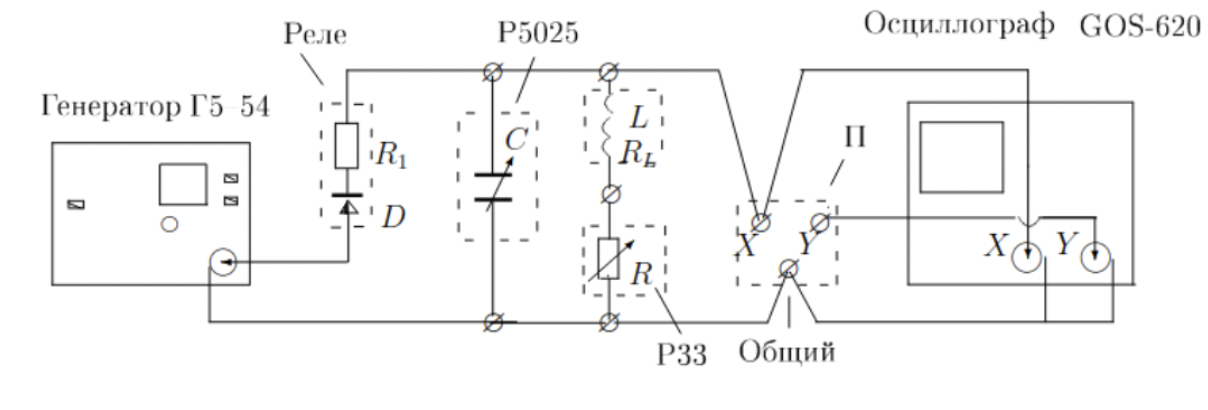
\includegraphics[width=\textwidth]{scheme.png}
    \caption{Схема экспериментальной установки}
    \label{fig:sheme}
\end{figure}

\section{Ход работы:}
\subsection{Измерение периодов свободных колебаний} \label{sec:T}

Соберём cхему, изображённую на Рис. \ref{fig:sheme}.Установим на магазине сопротивлений \(R = 0\); На магазине емкостей
величину \( C = 0.02\; мкФ \). Установим выходное напряжение генератора на \( 28\; V \). По ЭО измерим расстояние между соседними
импульсами \( (x_0 = 2.1 \cdot 5\; мс = 10.5\; мс ) \).

Будем измерять по ЭО расстояние \( x \) , которое занимают \( n \) полных периодов колебаний. Зная период задающих
колебания импульсов \( ( T_0 = 0.01\; с ) \) и \( x_0 \) можно расчитать период колебаний контура \( T \) по формуле:

\[ T = T_0x/(nx_0) \]

Проведём эти измерения изменяя емкость \( C \) от \( 0.02\; мкФ \) до \( 0.9\; мкФ \):

\begin{table}[H]
    \centering
    \label{table:T}
    \begin{tabular}{|c|c|c|c|c|c|c|}
    \hline
    \(C,\; мкФ \) & \(x_0,\; см\) & \(scale,\; мс\) & \(n\) & \(x,\; см\) & \(scale,\; мс\)& \(T,\; с\) \\\hline
    0.02   & 2.1    & 5         & 3 & 1     & 1         & 0.0006 \\\hline
    0.13   & 2.1    & 5         & 7 & 3     & 2         & 0.0106 \\\hline
    0.24   & 2.1    & 5         & 5 & 3     & 2         & 0.0274 \\\hline
    0.35   & 2.1    & 5         & 5 & 3.6   & 2         & 0.0480 \\\hline
    0.46   & 2.1    & 5         & 5 & 4.1   & 2         & 0.0718 \\\hline
    0.57   & 2.1    & 5         & 5 & 4.6   & 2         & 0.0999 \\\hline
    0.68   & 2.1    & 5         & 4 & 4     & 2         & 0.1295 \\\hline
    0.79   & 2.1    & 5         & 3 & 3.1   & 2         & 0.1555 \\\hline
    0.9    & 2.1    & 5         & 4 & 4.6   & 2         & 0.1971 \\\hline
    \end{tabular}
\end{table}

\subsection{Критическое сопротивление и декремент затухания} \label{sec:Rcr}
Приняв \( L = 200\; мГн \) рассчитаем ёмкость \( C \), при которой собственная частота колебаний контура 
\( \nu_0 = 1/(2\pi\sqrt{LC}) \) составляет \( 5\; kHz \):

\[ C = 0.005\; мкФ \]

Для полученных значений \( L \) и \( C \) рассчитаем критическое сопротивление контура \( R_{cr} \) по формуле:

\[ R_{cr} = 2\sqrt{L/C} = 12600\; Ом \]

Установим на магазине ёмкость, близкую к рассчитанной. Будем увеличивать \( R \) от \( 0 \) до \( R_{cr} \). Определим
сопротивление магазина \( R_0 \), при котором контур переходит в апериодический режим:

\[ R_0 = 7400\; Ом \]

Установим сопротивление \( R \simeq 0.1R_0 \) и будем измерять логарифмический декремент затухающих колебаний
по формуле:

\[ d = \frac{1}{n}\ln \frac{U_k}{U_{k+n}} \]

Повторим эти измерения для разных \( R \) от \( 0.1R_0 \) до \( 0.3R_0 \):

\begin{table}[H]
    \centering
    \begin{tabular}{|c|c|c|c|c|}
    \hline
    \(R,\; Ом\) & \(n\) & \(U_k,\; см \)& \(U_{k+n},\; см\) & \(d\) \\\hline
    740   & 3 & 4    & 1          & 0.462 \\\hline
    986   & 3 & 3    & 0.5        & 0.597 \\\hline
    1232  & 2 & 2.2  & 0.5        & 0.741 \\\hline
    1478  & 2 & 4    & 0.6        & 0.949 \\\hline
    1724  & 2 & 3.4  & 0.4        & 1.070 \\\hline
    1970  & 2 & 3    & 0.3        & 1.151 \\\hline
    \end{tabular}
\end{table}

\subsection{Свободные колебания на фазовой плоскости} \label{sec:d}
Подключим на ЭО канал Y, на который подано напряжение \( U_R \). Зафиксируем картину:

\begin{figure}[H]
    \centering
    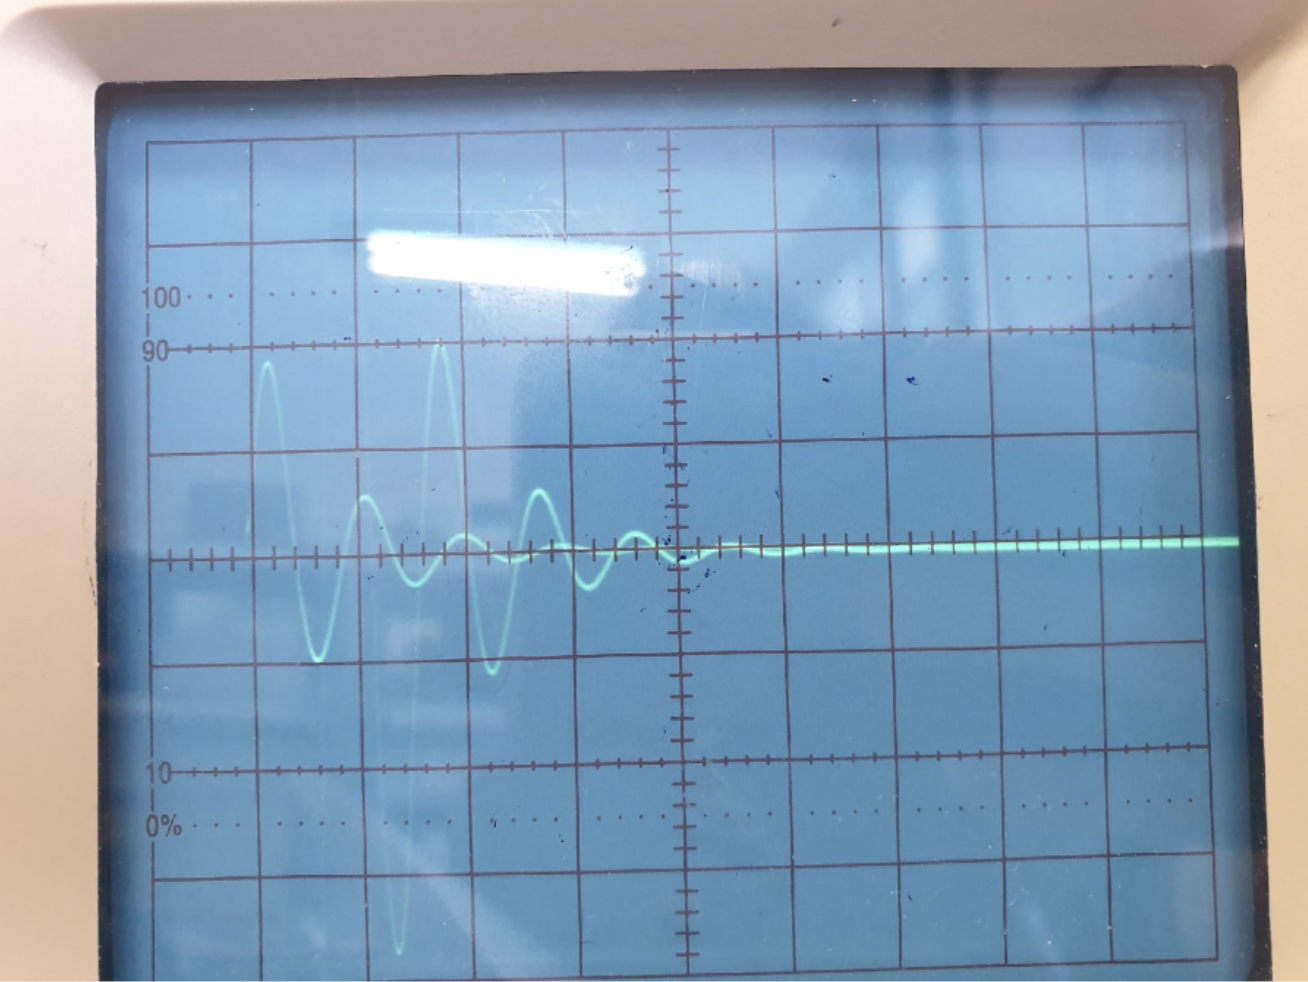
\includegraphics[width = 0.8\textwidth]{X_and_Y_time.jpg}
    \caption{Сигналы X и Y в развёртке по времени}
    \label{fig:XY_time}
\end{figure}

Отключим развёртку по времени, переведы ручку "TIME/DIV" в положение "X-Y".
Будем наблюдать за изменением картины при изменении \( R \) от \(0.1R_0\) до \(0.3R_0\):

\begin{figure}[H]
    \centering
    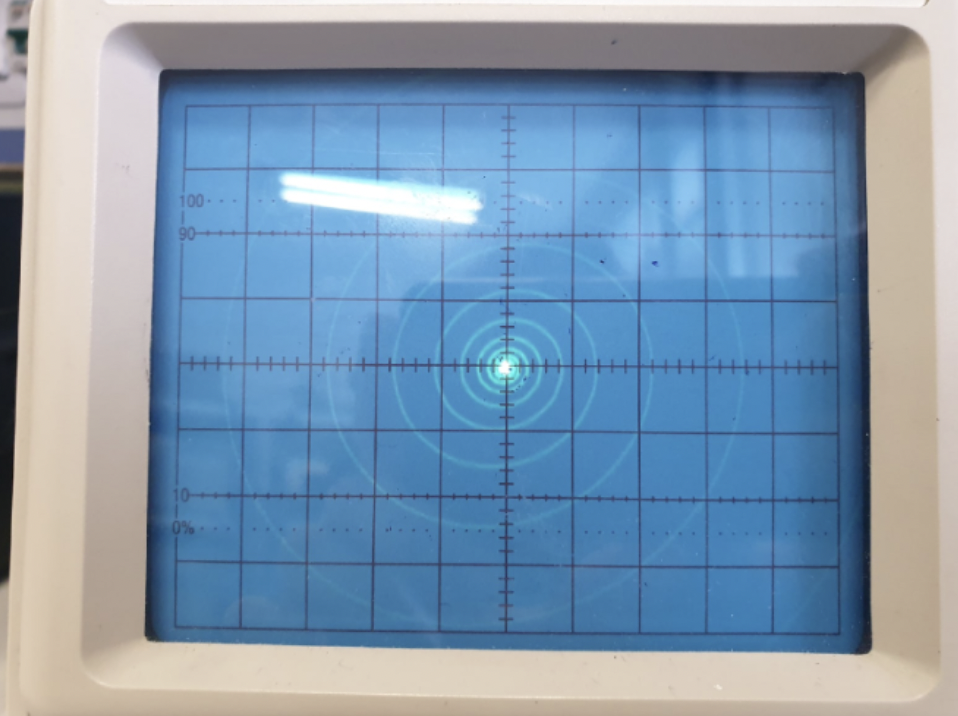
\includegraphics[width = 0.6\textwidth]{XY-740.jpg}
    \caption{Фазовая картина при \(R = 740\; Ом \)}
    \label{fig:XY_time}
\end{figure}
\begin{figure}[H]
    \centering
    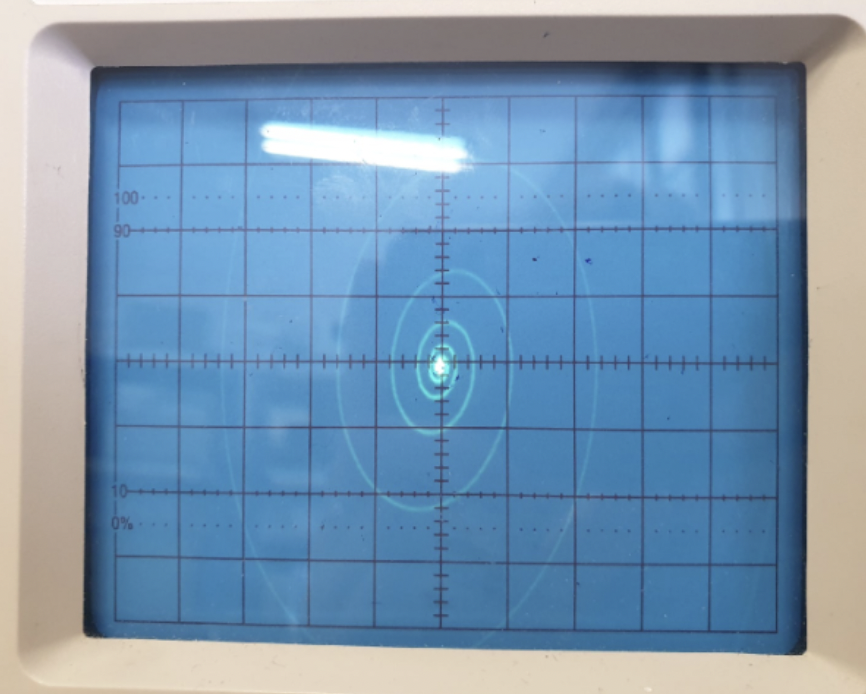
\includegraphics[width = 0.6\textwidth]{XY-1478.jpg}
    \caption{Фазовая картина при \(R = 1478\; Ом \)}
    \label{fig:XY_time}
\end{figure}
\begin{figure}[H]
    \centering
    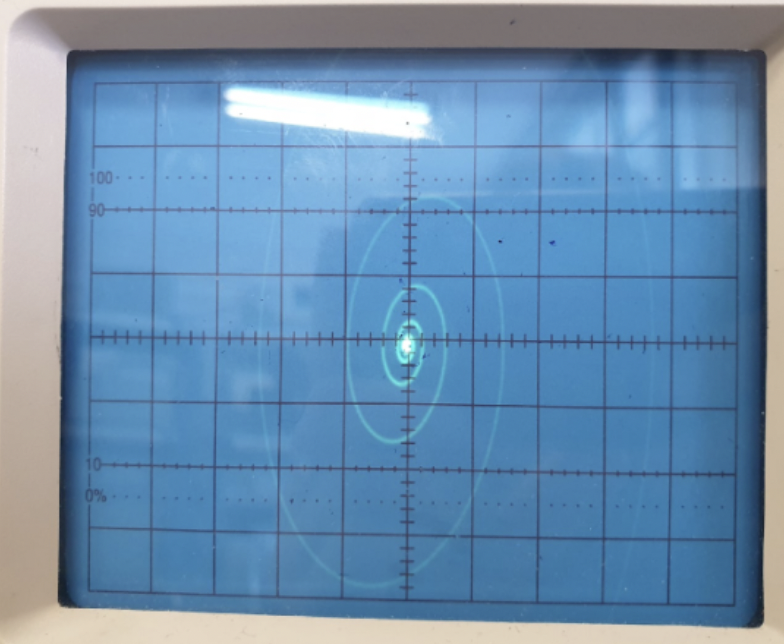
\includegraphics[width = 0.6\textwidth]{XY-1970.jpg}
    \caption{Фазовая картина при \(R = 1970\; Ом \)}
    \label{fig:XY_time}
\end{figure}

Измерим логарифмический декремент \(d\) контура для максимального и минимального значений \(R\) по формуле:

\[ d = \frac{1}{n}\ln\frac{x_k}{x_{k+n}} \]

\begin{table}[H]
    \centering
    \begin{tabular}{|c|c|c|c|c|}
        \hline
    \(R,\; Ом\) & \(n\) & \(X_k,\; см\) & \(X_{k+n},\; см\) & \(d\) \\\hline
    740  & 2 & 3.5 & 1.4 & 0.458 \\\hline
    1970 & 1 & 2.0 & 0.6 & 1.204 \\\hline
    \end{tabular}
\end{table}

Разберём цепь, отключим катушку и измерим её индуктивность \(L\) и оммическое сопротивление \(R_L\) при помощи
RLC-метра. Получим значения:
\[ L = 146\; мГн;\: R_L = 14\;Ом \]

\section{Обработка экспериментальных данных}
\subsection{Сравнение экспериментальных и теоретических значений периода T} \label{sec:T-T}

По формуле \( T = 2\pi\sqrt{LC} \) рассчитаем теоретические значения периодов для контура. и сравним с экспериментальными,
измеренными в пункте \ref{sec:T}:

\begin{table}[H]
    \centering
    \begin{tabular}{|c|c|}
        \hline
        \(T_{mes},\; 10^5 с\) & \(T_{th},\; 10^5c\) \\\hline
        31.7    & 33.8 \\\hline
        81.6    & 86.5 \\\hline
        114     & 118  \\\hline
        137     & 142  \\\hline
        156     & 163  \\\hline
        175     & 181  \\\hline
        190     & 198  \\\hline
        197     & 213  \\\hline
        219     & 228  \\\hline
    \end{tabular}
\end{table}

\begin{figure}[H]
    \centering
    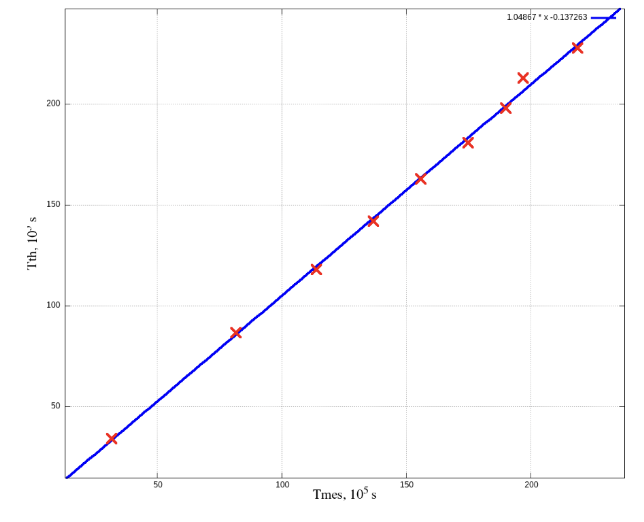
\includegraphics[width=0.8\textwidth]{T-T-res.png}
    \caption{График \(T_{th}\) от \(T_{mes}\)}
    \label{fig:T-T}
\end{figure}

Получили зависимость:
\[ T_{th} = a\cdot T_{mes} + b\]
\[ a = 1.05 \pm 0.01 \]
\[ b = -0.137 \pm 0.8\; с \]

Из апроксимации видно, что экспериментальные данный практически идеально совпадают с теоретическими.
\subsection{Декремент затухания и \(R_{cr}\)}
Используя данные из пункта \ref{sec:d} построим зависимость \( Y = f ( X ) \),
\(Y = 1/d^2\; X = 1/R_{\Sigma}\):
\begin{figure}[H]
    \centering
    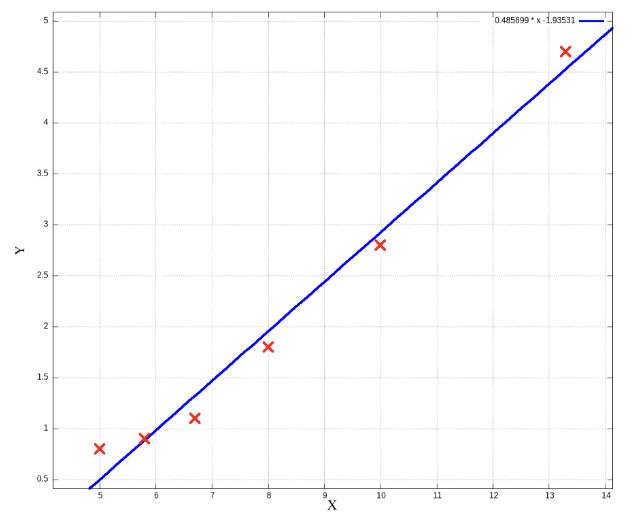
\includegraphics[width=0.8\textwidth]{d.png}
    \caption{График \(Y\) от \(X\cdot 10^4\)}
    \label{fig:d}
\end{figure}

По наклону графика в начале координат определим \(R_{cr}\):
\[ R_{cr} = 2\pi\sqrt{\Delta Y / \Delta X} = 264\; Ом \]

Видно, что это значение очень плохо совпадает со значениями, полученными в пункте \ref{sec:Rcr}. что говорит о
том, что данные способ определения критического сопротивления слабо соответствует реальности.

\subsection{Добротность} \label{sec:Q}
Расчитаем добротность для минимального и максимального значения \(R\), измеренных в пункте \ref{sec:d}. Используем формулу:
\[ Q = \frac{\pi}{d} \]
\begin{table}[H]
    \centering
    \begin{tabular}{|c|c|c|c|}
        \hline
    \(R,\; Ом\) & \(d\) & \( Q_{mes} \) & \(Q_{th}\)\\\hline
    740  & 0.458 & 6.9 & 8.5 \\\hline
    1970 & 1.204 & 2.6 & 3.2 \\\hline
    \end{tabular}
\end{table}

Видим, что экспериментальные данные довольно точно совпадают с теоретическими.
\section{Выводы}

В ходе лабораторной работы были измерены периды колебания контура, полученные значения совпадают с теоретическими в пределаъ погрешности; был проверен способ определения критического сопротивления \(R_{cr}\) через коэффициент наклона графика
\(1/d^2\) от \(1/R_{\Sigma}\). Полученные значения не совпадают с теоретическими (\(264\; Ом\) vs \(12600\; Ом\)). Были экспериментально получены значения добротности для контура при двух значениях \(R\). Полученные значения примерно совпадают с теоретическими. 

\end{document}

